	Revisiting our original research questions:

\begin{itemize}
	\item \emph{How effective are Machine Learning algorithms at predicting sentiment about weather?}
		In conclusion, we were able to successfully build a classifier that predicts the “sentiment”, “when” and “kind” for a given tweet. We approached the problem with three different learning algorithms: decision trees, Naïve Bayes and SVMs, which all performed better than the baseline. We also attempted a more advanced algorithm that used Markov Random Fields to factor in location data (which can be explored more in the future). 
	\item \emph{How do different algorithms compare in classifying tweets?}
	When comparing the different algorithms we saw that the Naïve Bayes classifier performed the best for predicting the sentiment of a tweet, while decision trees performed the best for predicting the “kind” of weather for a tweet. All three algorithms had a high accuracy for classifying the “when” of a tweet, however they did not perform much better than the baseline.
	\item \emph{How do we tailor our twitter data to reduce noise and extract the best features?}
	By preprocessing the data to remove stopwords, and by determining the most important words for each class, we were able to remove noise from our training data and keep our discriminative algorithm more efficient.
	\item \emph{Is Twitter a valuable source of information about public sentiment?}
	This is still very much up for discussion. The accuracy with which we were able to classify sentiment seems to indicate that Twitter data may actually be useful as a source of information on public opinion. For sake of illustration, we present the a heat map of the average sentiments for each of the 50 states, shown below. How much can we believe this information? Are people in the south less tolerant of poor weather, and thus complain more? Are people in Alaska as content as they claim to be? The data is here in plain sight -- the onus is now on us to decide what we want to believe. 
\end{itemize}

%HEAT MAP
\begin{figure}[!htb]
\noindent\makebox[\textwidth][c]{%
\minipage{0.75\textwidth}%
  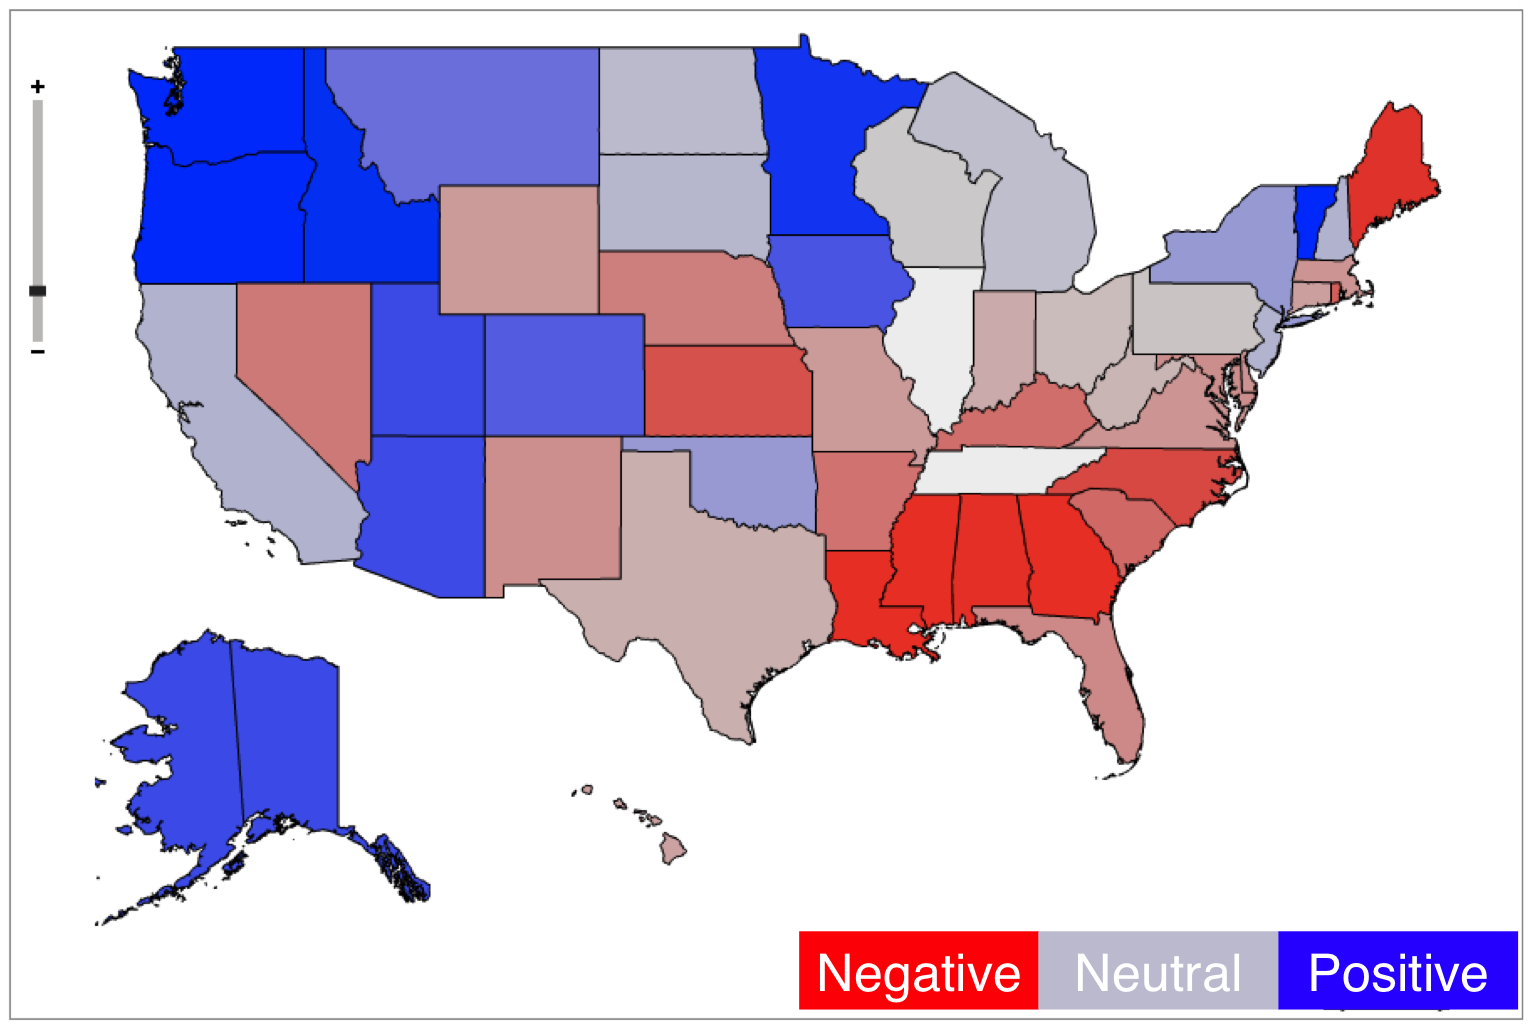
\includegraphics[width=\linewidth]{results/heatmap}
  \caption{Average ``Sentiments'' of the United States}\label{fig:heatmap}
\endminipage}
\end{figure}